\section{Analysis and Future Directions}
We first present a statistical analysis of the papers 
covered in this survey. Then, some future directions are proposed inspired by
our observations.
\begin{figure}[htbp]
	\centering
	\begin{minipage}[t]{0.45\linewidth}
		\centering
		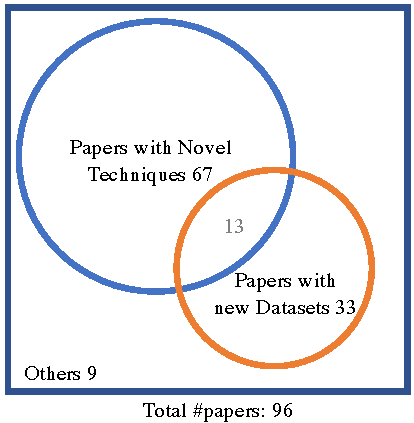
\includegraphics[scale=0.55]{fig/distribution1.pdf}
		\caption{Statistics of abstractive dialogue \\summarization papers.}
		\label{fig:papers}
	\end{minipage}
	\begin{minipage}[t]{0.45\linewidth}
		\centering
		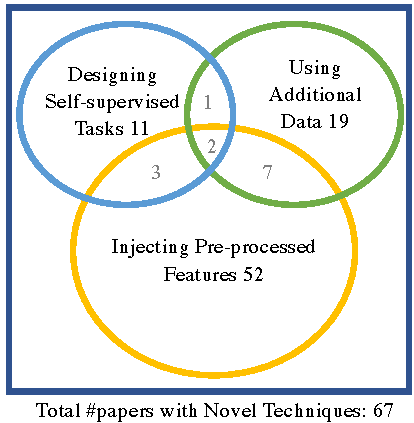
\includegraphics[scale=0.55]{fig/distribution2.pdf}
		\caption{Statistics of papers with technical contributions.}
		\label{fig:technical}
	\end{minipage}
\end{figure}
\subsection{Paper Analysis}\label{sec:observations}
The total number of papers on abstractive dialogue summarization investigated 
in this survey is $96$. 
As shown in Fig.~\ref{fig:papers}, $33$ of them propose new datasets and 
$67$ make novel technical contributions. The other $9$ papers are either 
a survey, a demo, or other strongly related papers. 
The overall ratio between technical papers and dataset papers 
(\textit{tech-data ratio}) is around $2.03:1$. Compared with the number of 
papers under different application scenarios in Fig.~\ref{fig:tech-data}, 
we found that scenarios of daily chat and official issues receive more 
attentions.
However, the other scenarios are less explored, with much lower 
tech-data ratios ranging from $1.0$ to $1.75$.
There is no significant difference in the number of datasets between
well-researched domains and the others. However, the release time and availability of different datasets vary.
AMI and ICSI are well-known meeting summarization datasets released in the early stage of the $20$th century, while most other datasets have been proposed in recent years.
Datasets for daily chat are all publicly available, while datasets for medical care and laws are not accessible to the majority of researchers. It's a good sign that high-quality corpora, such as AMI and SAMSum, lead to a prosperous of techniques for dialogue summarization, but also raise a worry about the generalization ability of current techniques because of their over-reliance on specific datasets which may lead to over-fitting.


The distribution of technical papers in each of the three research directions 
is shown in Fig.~\ref{fig:technical}.
While $11$ and $19$ papers focus on designing self-supervised tasks and 
using additional data, respectively, 
more than $77\%$ of the entire body of works targets the injection of 
pre-processed features. The trends of paper account for different techniques 
across scenarios that are similar to each other according to Fig.~\ref{fig:tech-scenario}.
The number of papers using features under different categories is 
shown in Fig.~\ref{fig:feature-scenario}, and we go for a deep insight into 
correlations between features and applications scenarios by categorizing 
papers according to features and their tested scenarios in 
Table~\ref{tab:correlation}. 

\begin{figure}[ht]
	\centering
	\subfigure[]{
	\begin{minipage}[t]{0.3\linewidth}
	\centering
	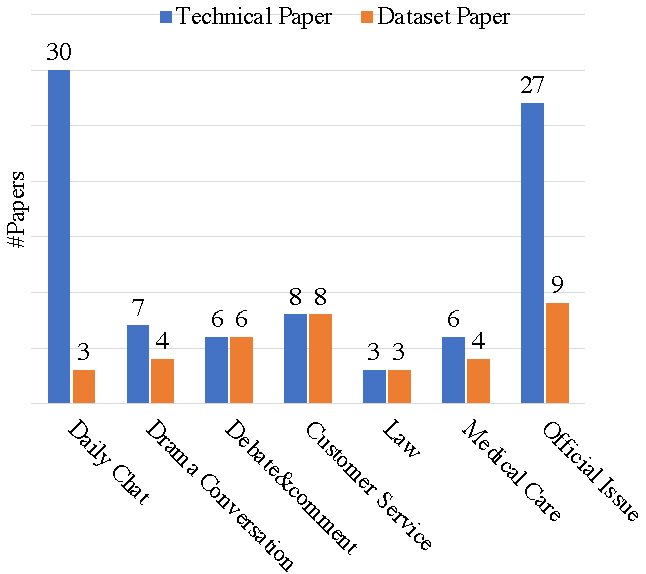
\includegraphics[scale=0.34]{fig/tech-data.pdf}
	\label{fig:tech-data}
	\end{minipage}}
	\subfigure[]{
	\begin{minipage}[t]{0.3\linewidth}
	\centering
	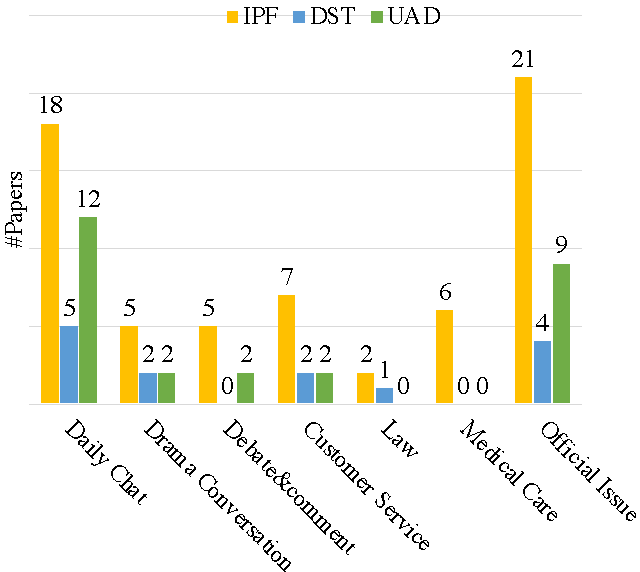
\includegraphics[scale=0.34]{fig/tech-scenario.pdf}
	\label{fig:tech-scenario}
	\end{minipage}}
	\subfigure[]{
	\begin{minipage}[t]{0.3\linewidth}
	\centering
	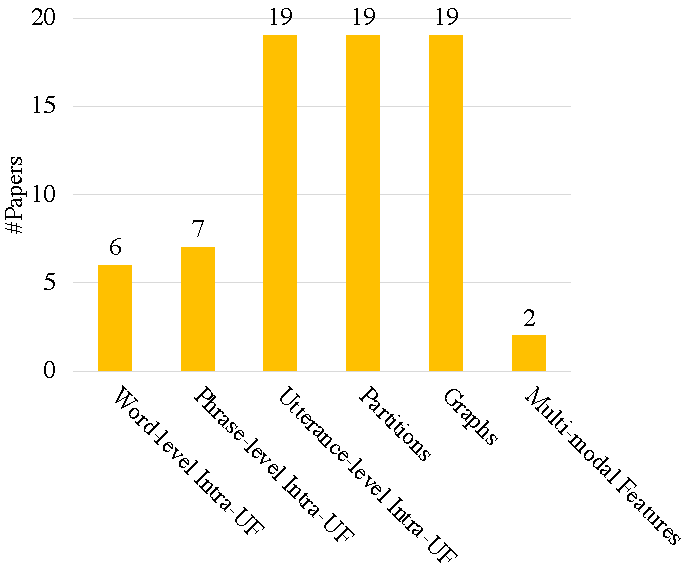
\includegraphics[scale=0.34]{fig/feature-scenario.pdf}
	\label{fig:feature-scenario}
	\end{minipage}}
\caption{(a) The number of technical papers and dataset papers under different scenarios. (b) The number of technical papers dividing by directions under different scenarios. IPF, DST and UAD are short for the three directions. (c) The number of technical papers under different features. Intra-UF is intra-utterance features.}
\end{figure}



\begin{table}
	\centering
	\scriptsize
	\caption{Existing work on injecting pre-processed features for 
		different scenarios. The taxonomy of features and dialogue summarization 
		scenarios are in the columns and rows respectively. A work may appear 
		multiple times since it experimented with 
		datasets under various scenarios or utilized features in different groups.}
	\begin{tabular}{|l|ccc|cc|c|}
		\toprule
		\multicolumn{1}{|c|}{\multirow{2}{*}{\diagbox{Scenarios}{Features}}} & \multicolumn{3}{c|}{\textbf{Intra-Utterance Features}} &\multicolumn{2}{c|}{\textbf{Inter-Utterance Features}} & \multirow{2}{*}{\textbf{\makecell{Multi-\\modal\\ Features}}} \\
		
		& \makecell[c]{Word\\level} & \makecell[c]{Phrase\\level} & \makecell[c]{Utterance\\level} & Partitions & Graphs& \\
		
		\midrule
		\multicolumn{7}{|l|}{\textit{Open-domain Dialogue Sumamrization}}\\
		\hline
		
		\makecell{Daily Chat}
		&\makecell{\cite{prodan2021prompt}} 
		&\makecell{\cite{feng2021language}\cite{khalifa2021bag}\\\cite{park2022unsupervised}\cite{wu2021controllable}}
		&\makecell{\cite{asi2022end}\cite{feng2021language}\cite{kim2022mind}\\\cite{lei2021hierarchical}\cite{lei2021finer}\cite{prodan2021prompt}\\\cite{wu2021controllable}\cite{zechner2002automatic}} 
		&\makecell{\cite{asi2022end}\cite{chen2020multi}\\\cite{feng2021language}\cite{liu2021topic}} 
		& \makecell{\cite{chen2021structure}\cite{feng2021incorporating}\cite{lei2021finer}\\\cite{liu2021controllable}\cite{liu2021coreference}\cite{park2022unsupervised}\\\cite{zhao2021give}\cite{liu2023picking}}
		&\makecell{-}\\

		
		\hline
		\makecell{Drama Conversation}
		&\makecell{-} 
		&\makecell{\cite{park2022unsupervised}}  
		&\makecell{-}  
		&\makecell{\cite{li2021hierarchical}\cite{liu2021topic}\cite{zhang2021summ}} 
		& \makecell{\cite{park2022unsupervised}\cite{zhao2021give}} 
		&\makecell{-}  \\

		
		\hline
		\makecell{Debate \& Comment}
		&\makecell{-} 
		& \makecell{\cite{park2022unsupervised}} 
		&\makecell{\cite{yang2022tanet}}  
		&\makecell{-}  
		&\makecell{\cite{chen2021structure}\cite{fabbri2021convosumm}\\\cite{feng2021incorporating}\cite{park2022unsupervised}\cite{yang2022tanet}} &\makecell{-}  \\
		
		
		\hline	 
		

		\multicolumn{7}{|l|}{\textit{Task-oriented Dialogue Sumamrization}}\\
		\hline
		
		\makecell{Customer Service}
		& \makecell{-}
		&\makecell{\cite{zou2021topic}} 
		& \makecell{\cite{asi2022end}\cite{yang2022tanet}\cite{yuan2019scaffolds}\\\cite{zhang2020unsupervised}\cite{zou2021topic}}
		& \makecell{\cite{asi2022end}\cite{zou2021unsupervised}}
		&  \makecell{\cite{yang2022tanet}\cite{yuan2019scaffolds}\cite{zhao2021todsum}}
		&  \makecell{-} \\

		
		\hline
		\makecell{Law}
		& \makecell{-} 
		& \makecell{\cite{gan2021inspectional}} 
		&\makecell{\cite{duan2019legal}\cite{gan2021inspectional}} 
		& \makecell{-}
		&  \makecell{-}
		& \makecell{-} \\

		
		\hline
		\makecell{Medical Care}
		&\makecell{-} 
		&  \makecell{\cite{joshi2020dr}}
		&\makecell{\cite{song2020summarizing}} 
		&\makecell{\cite{krishna2021generating}\cite{liu2019topic}\cite{zhang2021leveraging}} 
		&  \makecell{\cite{molennar2020healthcare}}
		& \makecell{-}\\

		
		\hline
		\makecell{Official Issue\\(Meeting\&Email)}
		&\makecell{\cite{murray2005extractive}\cite{OyaMCN14}\cite{qi2021improving}\\\cite{singla2017spoken}\cite{zhu2020end}} 
		&\makecell{\cite{feng2021language}\cite{park2022unsupervised}} 
		&\makecell{\cite{di2020da}\cite{feng2021language}\cite{goo2018abstractive}\\\cite{murray2005extractive}\cite{qi2021improving}\cite{yang2022tanet}\\\cite{zhu2020end}} 
		&\makecell{\cite{banerjee2015generating}\cite{di2020da}\cite{feng2021language}\\\cite{koay2021sliding}\cite{li2019keep}\cite{liu2021dynamic}\\\cite{qi2021improving}\cite{shang2018unsupervised}\cite{zhang2021summ}\\\cite{zheng2020abstractive}\cite{zhong2021qmsum}} 
		&\makecell{\cite{banerjee2015generating}\cite{feng2020dialogue}\cite{ganesh2019restructuring}\\\cite{MehdadCTN13}\cite{OyaMCN14}\cite{park2022unsupervised}\\\cite{shang2018unsupervised}\cite{yang2022tanet}} 
		&\makecell{\cite{li2019keep}\cite{murray2005extractive}}\\
		
		
		\bottomrule

	\end{tabular}
	\label{tab:correlation}
\end{table}


We make following observations:
\begin{itemize}

	\item Scenarios of Official Issue and Daily Chat attracted the most 
	attentions while other scenarios lack research as mentioned before. 

		\item Utterance-level intra-utterance features and inter-utterance 
	features are widely exploited, indicating that modeling utterance-level or 
	beyond utterance-level features is more effective for dialogue 
	understanding. Among them, speaker/role information and topic transitions are 
	two features which work well 
	under both ODS and TDS scenarios. There is also a lack of attention on 
	multi-modal features, possibly due to the scarcity of multi-modal datasets.

		\item Word-level and phrase-level intra-utterance features are no longer
	required with the wide adoption of pre-trained language models, except in
	integrating domain dictionaries in TDS. These features, especially keywords,
	are preferred to use as nodes for further constructing graphs, which helps 
	capture the global information flows for both ODS and TDS. 

		\item Partitions are extremely effective for TDS where dialogues 
	are usually long with inherent semantic transitions, such as agendas for meetings and domain shifts in customer service. 
	Identifying these transitions achieves a high degree of consensus among annotators. 
	In contrast, semantic flows in ODS are often interleaved in a complex fashion,
	which can be better represented as graphs, such as discourse graphs and topic graphs.

\end{itemize}




